%!TEX root = main.tex
\section{Background and Motivation}
\label{sec:background}

\subsection{LLM Applications: A Primer}
\label{sec:applications}

\subsubsection{The trend towards LLM applications.} 
Large language models (LLMs)~\cite{brown2020language,floridi2020gpt,touvron2023llama} stand out as a general technique whose intelligence capability can potentially be applied to various domains~\cite{dosovitskiy2020image,hadi2023survey}. 
Yet, even though AI models are evolving rapidly~\cite{sonoda2024diagnostic,reid2024gemini}, it is commonly recognized that a single LLM request is often deficient when addressing realistic problems. 
For example, the input context windows of typical LLMs are often of limited sizes (less than 10M tokens)~\cite{chen2023extending,lin2024infinite}, thus processing a large document would require issuing multiple parallel inference requests. 
Meanwhile, LLMs are plagued by the problem of \emph{hallucination}~\cite{ji2023survey}, meaning that the output of a single LLM request may be unfaithful or nonsensical, and some additional LLM requests are then required to ensure LLM output quality (for example, with FacTool~\cite{chern2023factool} verifications or with self-reflection~\cite{ji2023towards}).
Besides, the built-in knowledge and capability of LLMs are usually insufficient in professional occasions, thus various non-LLM components (e.g., knowledge retrieval~\cite{lewis2020retrieval}, third-party tools~\cite{shen2024llm} or other small models~\cite{shen2024hugginggpt}) are commonly adopted to augment LLM capabilities~\cite{abhyankarinfercept}, as 
%such functionalities are commonly 
integrated in LLM agents like AutoGPT~\cite{fezari2023gpt} and MetaGPT~\cite{hong2023metagpt}. 
To summarize, to enlarge the input length, improve the output reliability, and integrate more functionalities, LLM practitioners often need to conduct multiple inferences with the necessary non-LLM computations, which form a compound workflow.
% \ys{What exactly are LLM applications? Is LLM-based chat an LLM app? Yes, it is. I think the main trend is that to mitigate LLM hallucination and to improve AI accuracy at complex reasoning tasks, LLM-based apps have evolved from single-turn LLM-based chat to a more compound and complicated workflow. Then list examples such as RAG, o1, factool etc.}

We call the above compound workflow---with multiple LLM requests and even non-LLM tasks to accomplish a realistic mission---as an \emph{LLM application}.
LLM applications are rapidly emerging in recent years~\cite{hadi2023survey,tan2024teola,lin2024parrot}, and have become an increasingly prevalent workload type in production clusters.
Fig.~\ref{fig:app_structure} presents the structures and descriptions of ten typical LLM applications\footnote{
We deem multi-turn conversation as a special application whose mission is to help users obtain the desired information via iterative LLM interaction.
Moreover, in solution design, we do not particularly differentiate AI agents~\cite{fezari2023gpt,hong2023metagpt} from other applications, because the definition of agent itself is vague, and the typical components of AI agents, like ReActing, planning, RAG, and tool-calling, have all been considered in our modeling of LLM applications.
Finally, we admit that it is impossible to exhaustively list all the LLM applications here, but we believe the applications in Fig.~\ref{fig:app_structure} are sufficiently representative because they cover the essential characteristics of general LLM applications (as summarized later in Table 1). 
}
studied in this paper.


\begin{figure*}
    \centering
    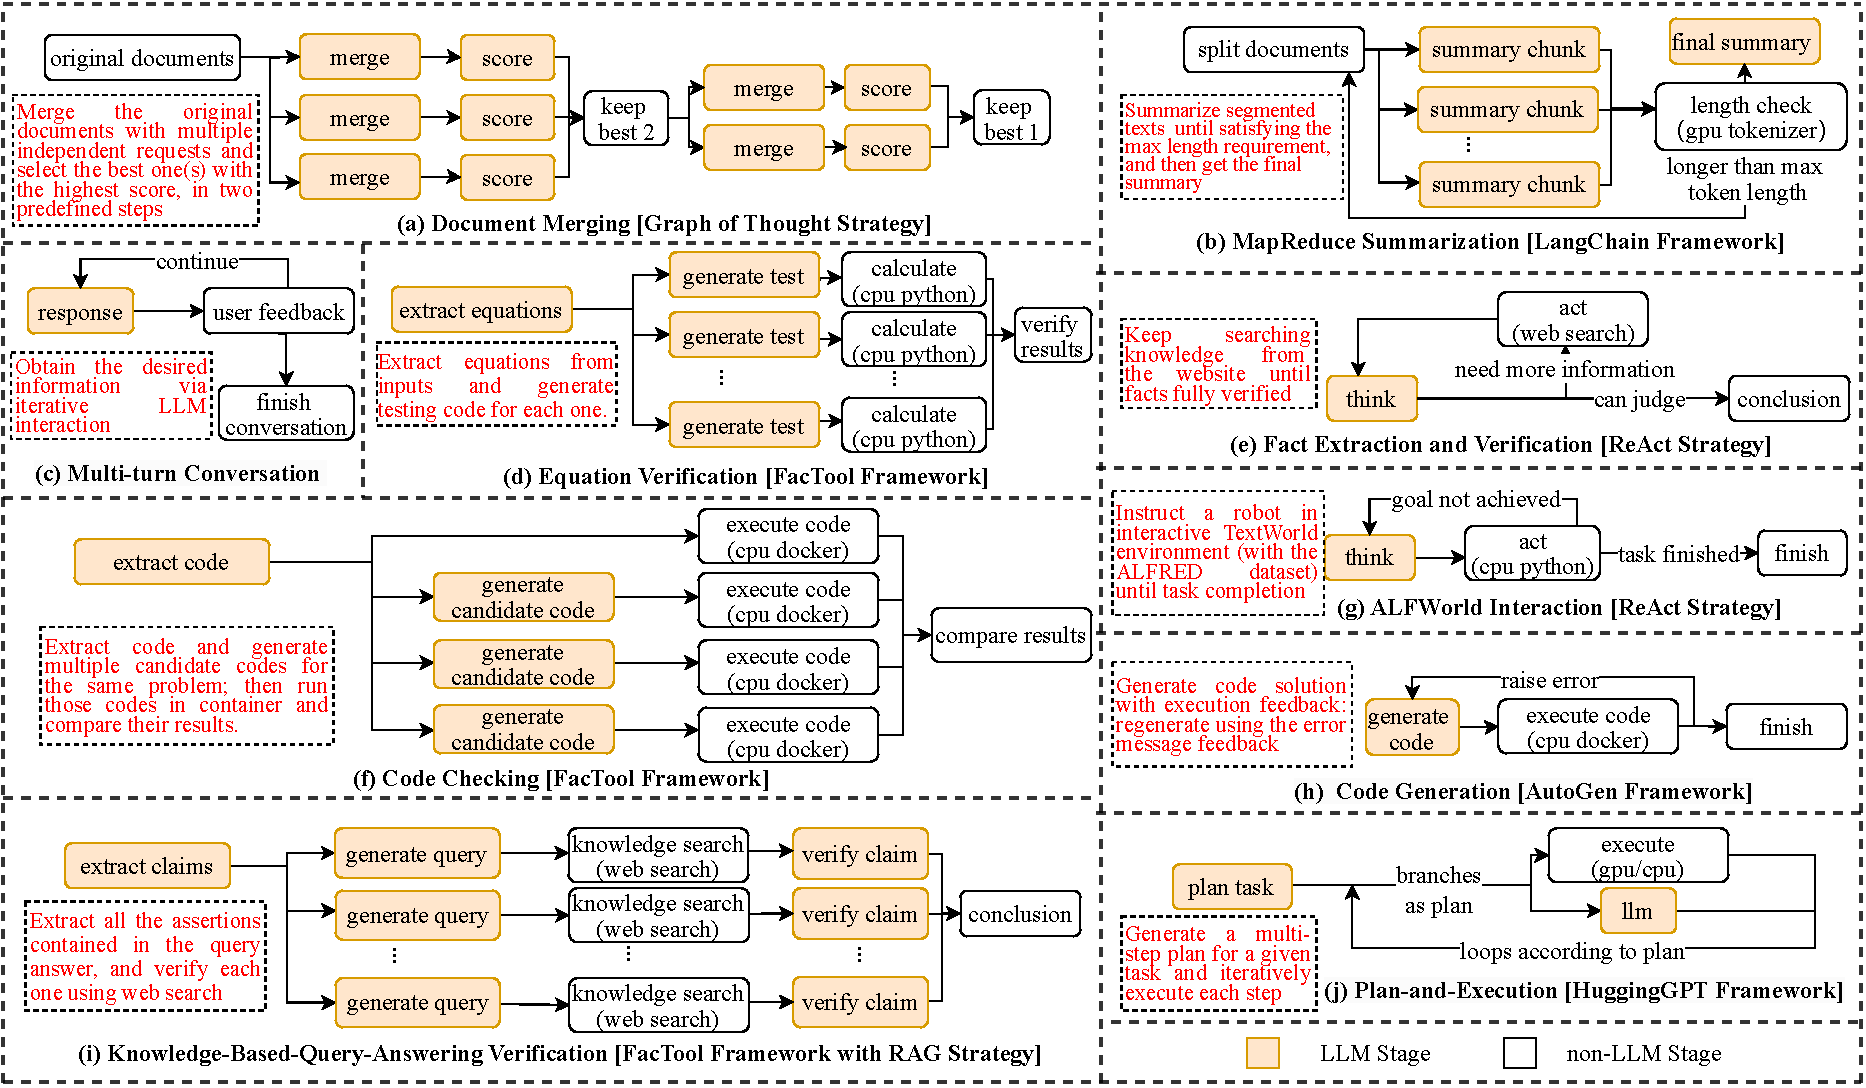
\includegraphics[width=0.96\textwidth]{figures/app structure.pdf}
    \caption{The structures of typical LLM applications (sources listed in Table 1). An application can be built with dedicated frameworks (e.g., FacTool and AutoGen) or following certain control strategies (e.g., Graph of Thought and ReAct). }
    %Used Applications. \chen{add brief introduction and source citation} \chen{add conversation and planning?} \chen{place description directly in figures? Summary the common patterns in title instead?} \gz{multi-turn conversation fault}}
    \label{fig:app_structure}
    \vspace{-0.1in}
\end{figure*}

%\ys{For the following characteristics, we could add another subsection with the name like "Challenges of Compound LLM Applications". In all, this subsection is used to present challenges, aka motivation, problem statement of this paper.}
\subsubsection{Challenging characteristics of LLM applications.}
The serving quality of LLM applications is critical to user experience and the total service profit. 
Nonetheless, it is indeed quite challenging to efficiently serve the LLM applications given their distinct characteristics as follows:

 \emph{1) Demand Dynamicity.}
        The resource demand of LLM applications exhibits strong dynamicity on two levels. %both inter-request level and intra-request level.
        First, the application structure (i.e., the number and organization of the constituting requests) may be uncertain in advance.
        Although some applications (like the hard-coded inference workflows with LangChain~\cite{topsakal2023creating}) have a fixed structure, for some other applications with ReActing~\cite{ji2023towards,yao2022react} or LLM-planning~\cite{shen2024hugginggpt}, the application structure can only be determined at runtime based on the inference contents. 
        Second, for each individual request, as pointed out by many existing works~\cite{gao2024cost,wu2023fast}, both the input and output token lengths are dynamic.
        This implies that the inference duration and peak memory consumption (which are positively correlated with the number of tokens) are also difficult to predict a priori.
        
 \emph{2) Resource Hybridity.}
        While LLM inferences with GPU backends are the mainstream computations in LLM applications, there also exist various non-LLM tasks in many agent-like applications. 
	Those non-LLM tasks demand additional resources other than GPUs.
	For example, in the code-generation application provided by the FacTool framework, the LLM-generated codes need to be tested on CPU backends (e.g., with a        docker container~\cite{factool_code}). 
	Meanwhile, remote knowledge retrieval~\cite{lewis2020retrieval} would consume network resources. 
        Efficient serving of LLM applications would require coordinated provisioning of such hybrid resources. % need to be coordinated well for efficiently serve the LLM applications. 
        
 \emph{3) Objective Diversity.}
        Different LLM applications, based on their respective service contents, may have different performance objectives.
        For example, for many applications where only the final outputs matter---like document-summarization~\cite{jin2024comprehensive} or code-generation~\cite{autogen}, users only care about the ultimate application completion time.
        Meanwhile, applications may also have different service level objectives: for applications whose intermediate results need to be timely returned to users---like conversational text streaming services~\cite{liu2024andes}, the performance objective is to attain high instantaneous generation speed (as measured by the \emph{Time-To-First-Token} and \emph{Time-Per-Output-Token} metrics~\cite{zhong_distserve_2024}).
        In some other cases, the performance objective can also be to get the final output prior to the specified deadline~\cite{nie2024aladdin}. 
        We note that the performance objective is a built-in property of an LLM application, which shall be indiscriminately respected in scheduling.
        
In Table 1, we check each application in Fig.~\ref{fig:app_structure} against the above aspects, which suggests that those characteristics are quite common for modern LLM applications.
Note that such characteristics are significantly different from the traditional model serving workloads prior to the LLM era~\cite{crankshaw2017clipper,zhang2019mark} (which have fixed inference time, only consume GPU resources, and share the same performance objective).
In a nutshell, to design an ideal serving system for LLM applications, we need to properly deal with such distinct characteristics, seeking to yield high service quality at the application level---which is directly perceived by end users.
%ideal LLM serving system shall
%Confronting the above challenges, an ideal LLM serving system shall
%behave well in application-level service quality to guarantee the ultimate user experience.
%be able to yield high service quality at the application level for good user-perceptive experience.
%\ys{do we have experiments that can be used to motivate work? If so, we can put some here.}

\begin{table}
\centering
\resizebox{\linewidth}{!}{
\begin{tabular}{|c|c|c|c|c|c|c|c|c|}
\hline
\multirow{2}{*}{Task} & \multicolumn{3}{|c|}{Demand Dynamicity} & \multicolumn{2}{|c|}{Resource Hybridity} & \multicolumn{3}{|c|}{Objective Diversity}\\  \cline{2-9}
                                   & Structure & Parallelism & I/O              & GPU       & Non-LLM backends                      & ACT       & DDL       & TPT \\ \hline
(a) DM \cite{got_docmerge}        & \ding{55} & \ding{55}   & \ding{51}       & \ding{51} & \ding{55}       & \ding{51} & \ding{51} & \ding{55}  \\ \hline
(b) MRS \cite{Langchain_MapReduce} & \ding{51} & \ding{51}   & \ding{51}       & \ding{51} & \ding{51} (GPU: tokenizer)      & \ding{51} & \ding{51} & \ding{55}  \\ \hline
(c) MC \cite{sharegpt}            & \ding{51} & \ding{55}   & \ding{51}       & \ding{51} & \ding{55}       & \ding{55} & \ding{55} & \ding{51}  \\ \hline
(d) EV \cite{factool_math}        & \ding{55} & \ding{51}   & \ding{51}       & \ding{51} & \ding{55}      & \ding{51} & \ding{51} & \ding{55}  \\ \hline
(e) FEV \cite{react_fever}         & \ding{51} & \ding{55}   & \ding{51}       & \ding{51} & \ding{51} (Network: search)      & \ding{51} & \ding{51} & \ding{55}  \\ \hline
(f) CC \cite{factool_code}        & \ding{55} & \ding{55}   & \ding{51}       & \ding{51} & \ding{51} (CPU: docker)       & \ding{51} & \ding{51} & \ding{55}  \\ \hline
(g) ALFWI \cite{react_alfw}          & \ding{51} & \ding{55}   & \ding{51}       & \ding{51} & \ding{55}    & \ding{51} & \ding{51} & \ding{55}  \\ \hline
(h) CG \cite{autogen}             & \ding{51} & \ding{55}   & \ding{51}       & \ding{51} & \ding{51} (CPU: docker)       & \ding{51} & \ding{51} & \ding{55}  \\ \hline
(i) KBQAV \cite{factool_kbqa}        & \ding{55} & \ding{51}   & \ding{51}       & \ding{51}  & \ding{51} (Network: search)   & \ding{51} & \ding{51} & \ding{55}  \\ \hline
(j) PE \cite{hugginggpt}          & \ding{51} & \ding{55}   & \ding{51}       & \ding{51} & \ding{51} (GPU: small models)      & \ding{51} & \ding{51} & \ding{55}  \\ \hline
\end{tabular}
}

\vspace{0.1in}
\caption{
Characteristics in aspects of \emph{demand dynamicity}, \emph{resource hybridity} and \emph{objective diversity} for the LLM applications in Fig.~\ref{fig:app_structure} (for conciseness, hereafter we use the uppercase letter abbreviation to represent each application).
Regarding the objectives, ACT means to reduce Application Completion Time, DDL means to meet a preset completion deadline, and TPT means to guarantee the instantaneous performance on \emph{time per (processed) token} (for simplicity, here we do not differentiate prompt or completion tokens).
%The classification of applications. As seen in the table, our workloads cover all three different types of Demand Dynamicity and require backends using different resources. Moreover above applications have three different performance or service level objectives. So we could claim that our testbed is sound and diversity.(for conciseness, we use the uppercase letter abbreviation to represent each application), 
}
\vspace{-0.1in}
\end{table}

\subsection{Prior Arts and Their Limitations}

% \begin{figure}
%     \centering
%     \includegraphics[width=0.5\linewidth]{example-image-a}
%     \caption{request scheduling vs. good CoInference scheduling vs. bad CoInference scheduling}
%     \label{fig:toy_example}
% \end{figure}

% \ys{This is the background and motivation section not the Related Work section hence we should keep this simple so readers do not get lost. My suggestion is emphasize on works that deal with agent scheduling, inter-request scheduling etc. This is a relatively new field. I think only these papers qualify: Parrot and Teola. Experts will ask (a) what is the design space of agent/multiple-LLM scheduling; (b) WHY parrot and Teola cannot solve the challenges presented above; (c) finally, what's new with CoInfer and Hermes, what's our key insight.}

% In the literature, a bewildering array of research works have appeared on improving LLM inference performance.
% In \emph{operator implementation} aspect, the FlashAttention~\cite{dao2022flashattention} and FlashDecoding~\cite{hong2024flashdecoding} style algorithms are commonly adopted to realize efficient LLM inference by integrating IO awareness. 
% In \emph{model deployment} aspect, model-quantization~\cite{frantar2022gptq,kim2023squeezellm}, paged-attention~\cite{kwon2023efficient} and prefill-decode-separation~\cite{zhong_distserve_2024,agrawal_taming_2024} methods have been proposed to maximize backend utilization.
% In \emph{inference algorithm} aspect, continuous batching~\cite{yu_orca_2022} and speculative decoding methods~\cite{miao2023specinfer,cai2024medusa} are also applied to improve the inference throughput.
% In \emph{request scheduling} aspect, a series of request-level scheduling algorithms like FastServe~\cite{wu2023fast} and Llumnix~\cite{sun2024llumnix} have emerged to improve the overall serving performance. 
% Yet, those inference-level optimizations are oblivious to the correlation of the requests belonging to the same LLM application, often being sub-optimal in application-level performance. 

In the literature, many research works have been proposed on optimizing LLM inferences in aspects like operator implementation~\cite{dao2022flashattention,hong2024flashdecoding}, model deployment~\cite{frantar2022gptq,kim2023squeezellm,kwon2023efficient,zhong_distserve_2024,agrawal_taming_2024} and inference algorithm~\cite{yu_orca_2022,miao2023specinfer,cai2024medusa,wu2023fast,sun2024llumnix}.
%~\cite{dao2022flashattention,kim2023squeezellm,miao2023specinfer,sun2024llumnix,cai2024medusa}.
Nonetheless, they mostly focus on individual inference requests, being oblivious to the request correlations and often suffering sub-optimal application-level performance. 
In particular, when scheduling multiple requests, the default policy adopted in popular inference frameworks like vLLM~\cite{vllm} is First-Come-First-Serve (FCFS) (largely due to demand uncertainty). 
Fig.~\ref{fig:toy_example} shows two LLM applications (A and B) served by a LLM engine (which we assume can serve only one request at a time, i.e., with a batch size of 1).
The default request-level FCFS scheduler (Fig.~\ref{subfig:request-level fcfs}) would interleave the inference serving of different applications, leading to long average Application Completion Time (ACT).
However, if we prioritize all the inference requests of B over A (Fig.~\ref{subfig:prioritize B over A}), we can substantially reduce the average ACT. 
%\chen{So for the objectives on instantaneous time-per-output-token}
% \ys{probably should move this toy example and its test numbers to the Problem Statement part.}

\begin{figure}
    \vspace{-.18in}
    \centering
    \subfloat[\vspace{-0.1in}Request-level FCFS]
    {
        \label{subfig:request-level fcfs}
        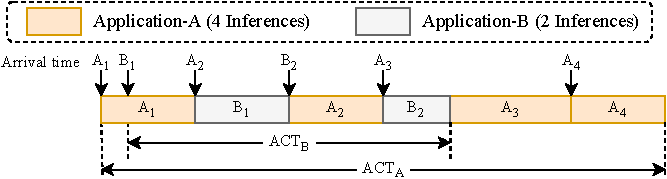
\includegraphics[width=6cm]{figures/scheduling_motivation/request_level_fcfs.drawio.pdf}
    }\hfill
    \subfloat[\vspace{-0.1in}Prioritize B over A]
    {
        \label{subfig:prioritize B over A}
        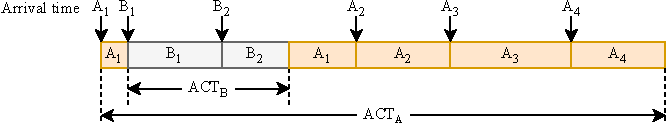
\includegraphics[width=6cm]{figures/scheduling_motivation/prioritize_b_over_a.drawio.pdf}
    }\hfill
    \subfloat[\vspace{-0.1in}Prioritize A over B]
    {
        \label{subfig:prioritize A over B}
        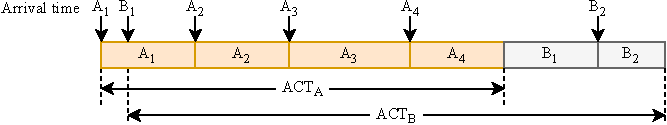
\includegraphics[width=6cm]{figures/scheduling_motivation/prioritize_a_over_b.drawio.pdf}
    }\hfill
    \caption{A toy example showing the scheduling algorithms' impact on the overall performance of two LLM applications (A and B, respectively with 4 and 2 dependent LLM requests indexed by the subscripts).
    Compared with request serving in FCFS (first-come-first-serve) manner, prioritizing all requests of B over A can yield a shorter average ACT (Application Completion time), yet an improper order (prioritizing A over B as in FCFS manner) leads to a worse performance.}
    \label{fig:toy_example}
\end{figure}

Apart from accelerating individual LLM inferences, there do exist some recent works on improving the performance of LLM applications.
For example, Parrot~\cite{lin2024parrot} employs a simple heuristic that schedules the requests of an application together to optimize the end-to-end performance. 
%proposes to identify the correlated inferences with the notion of semantic variables, and 
However, merely executing the correlated request together is not enough: as shown in Fig.~\ref{fig:toy_example}, the average ACT when instead prioritizing A over B (Fig.~\ref{subfig:prioritize A over B}) is even worse than the default case (Fig.~\ref{subfig:request-level fcfs}). 
%There are some other methods on application level optimizations: 
Apart from Parrot, CachedAttention~\cite{gao2024cost} and Infercept~\cite{abhyankarinfercept} focus on improving the effectiveness of KV-cache reusing between dependent requests of an LLM application; 
Teola~\cite{tan2024teola} applies compilation and batching optimizations to accelerate individual applications; 
Andes~\cite{liu2024andes} seeks to improve the instantaneous token generation performance for text streaming services. 

\begin{figure*}
            \vspace{-.1in}
	\parbox[t]{18cm}{
		\centering
		{
			\centering
			
\includegraphics[width=3.2cm]{figures/prompt/0.pdf}
			\label{fig:p_token_factoolcode}
		}\hfill
		{	
			\centering
			
\includegraphics[width=3.2cm]{figures/prompt/3.pdf}
			\label{fig:p_token_gotdecmerge}
		}\hfill
		{	
			\centering
			
\includegraphics[width=3.2cm]{figures/prompt/1.pdf}
			\label{fig:p_token_factoolkbqa}
		}\hfill
		{	
			\centering
			
\includegraphics[width=3.2cm]{figures/prompt/2.pdf}
			\label{fig:p_token_factoolmath}
		}\hfill
		{	
			\centering
			
\includegraphics[width=3.2cm]{figures/prompt/4.pdf}
			\label{fig:p_token_reactfever}
		}\hfill
     
		\subfloat[Code Checking]
		{
			\centering
			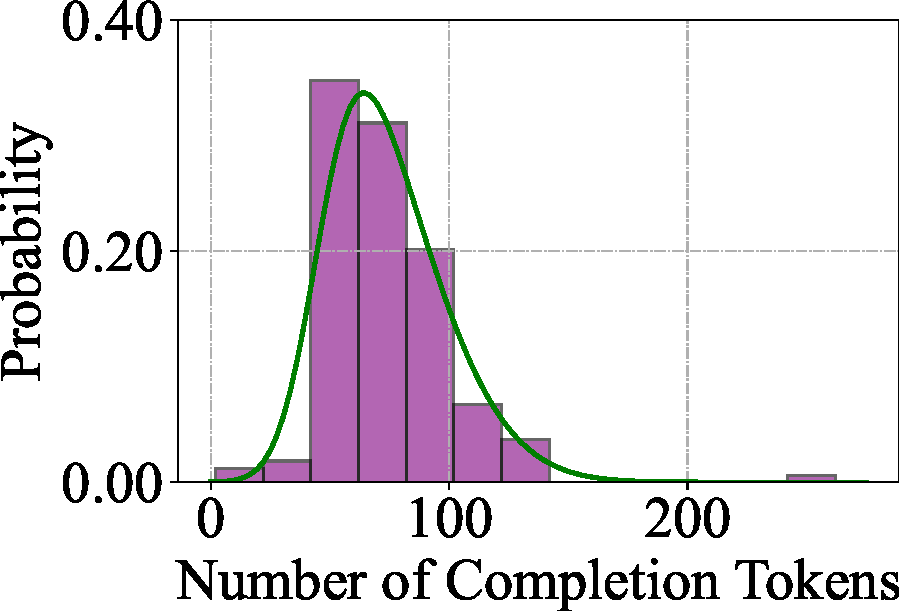
\includegraphics[width=3.2cm]{figures/completion/0.pdf}
			\label{fig:c_token_factoolcode}
		}\hfill
		\subfloat[Document Merging]
		{	
			\centering
			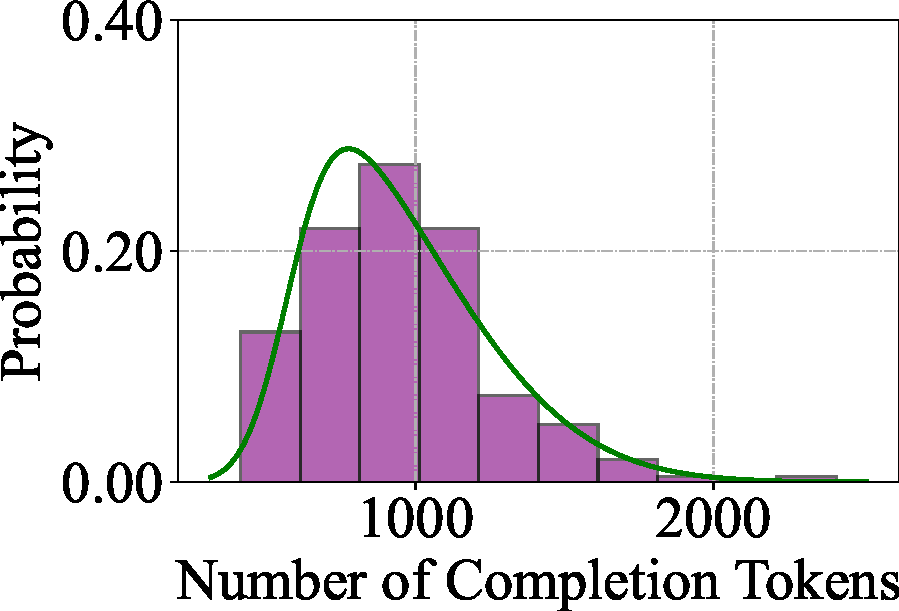
\includegraphics[width=3.2cm]{figures/completion/3.pdf}
			\label{fig:c_token_gotdecmerge}
		}\hfill
		\subfloat[KBQAV]
		{	
			\centering
			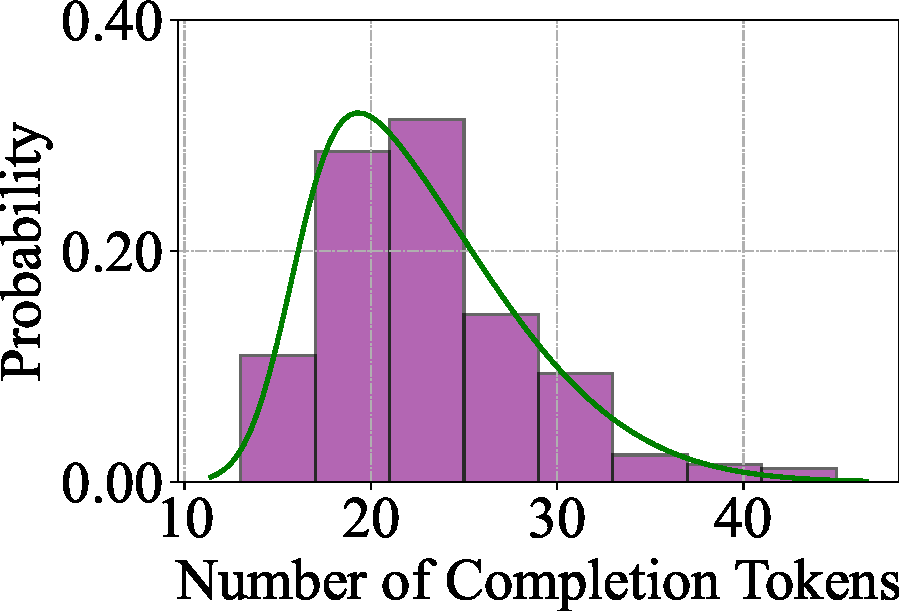
\includegraphics[width=3.2cm]{figures/completion/1.pdf}
			\label{fig:c_token_factoolkbqa}
		}\hfill
		\subfloat[Equation Verification]
		{	
			\centering
			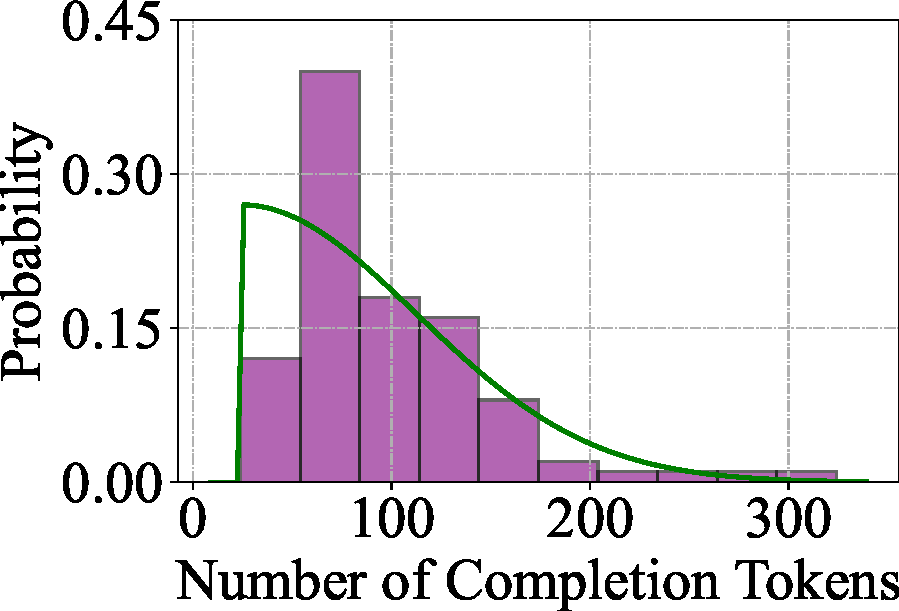
\includegraphics[width=3.2cm]{figures/completion/2.pdf}
			\label{fig:c_token_factoolmath}
		}\hfill
		\subfloat[Fact Extraction and Verification]
		{	
			\centering
			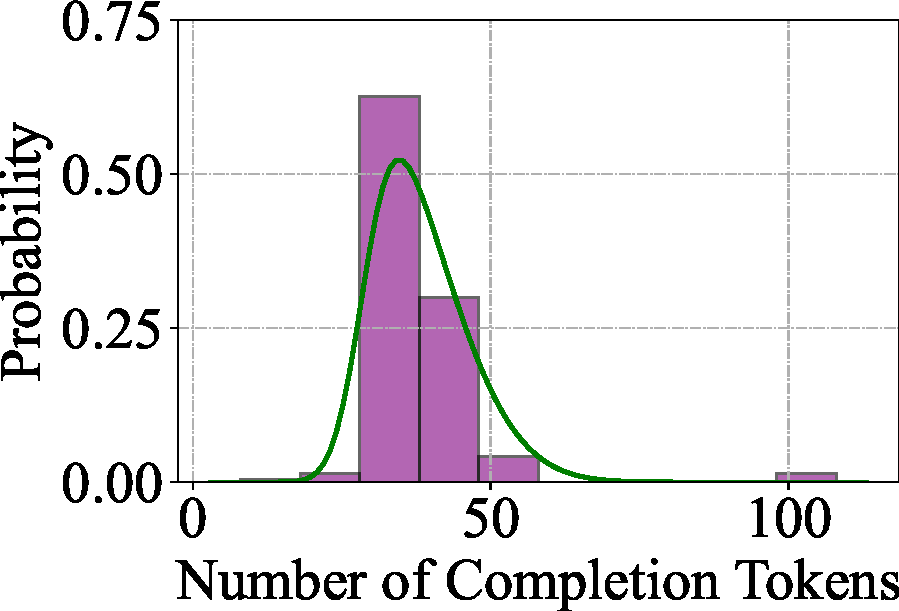
\includegraphics[width=3.2cm]{figures/completion/4.pdf}
			\label{fig:c_token_reactfever}
		}
            \vspace{-.1in}
		\caption{
                Prompt and completion token length distribution for an arbitrarily-selected request (marked at the top) in five applications each over 100 trial runs.
                In each case, we divide the length range into 10 buckets, and calculate the value appearance probability in each bucket (accompanied by the fitted curves assuming skewed Guassian distribution for reference).}
		\label{fig:token_usage}
	}
\end{figure*}


Nonetheless, although those works are application-aware, they largely ignore the three characteristics of LLM applications---by focusing on a single application structure (e.g., text streaming~\cite{liu2024andes}), a single resource type (e.g., KV-cache~\cite{gao2024cost}) or a single scheduling objective (e.g., end-to-end completion time~\cite{lin2024parrot}). 
There is a lack of a serving system designed for general LLM applications with their common characteristics properly handled, which further leads to two consequences.

First, due to the overwhelming demand dynamicity, it is hard to know the application-level resource consumption, rendering it difficult to improve the overall ACT with advanced scheduling algorithms like SRPT (letting alone to smoothly support diverse scheduling objectives).
Second, when serving LLM applications in the dark, it is hard to coordinately provision the desired resources on each backend, and a single LLM application---even when it is prioritized in the global queue---may still be impeded on any backend due to factors like cold cache, non-LLM resource contention and improper backend configuration (detailed later in \S\ref{subsec:resource_provisioning}).

% To summarize, although those works are application-aware, they largely ignore the three characteristics of LLM applications: they focus on a single application structure (e.g., text streaming~\cite{liu2024andes}), a single resource type (e.g., KV-cache~\cite{gao2024cost}) or a single scheduling objective (e.g., end-to-end completion time~\cite{lin2024parrot}). 
% There is a lack of a general serving system for LLM applications which can properly deal with their typical characteristics (dynamic demand structures, hybrid resource backends and diverse performance objectives).
% \chen{add more deficiencies}

% Moreover, as we shown later in Sec.X, request correlation awareness not only allows for scheduling at a coarser granularity, but also provides an opportunity to mitigate demand uncertainty---by referring to execution information of the requests in the previous rounds or even of the requests just-finished in the ongoing round. 
% Existing works fail to capture such opportunities and, when serving requests from general LLM applications, have to act in the dark and usually suffer compromised service quality.

\phm{Objective.}
Motivated by the deficiencies of existing works, our objective in this paper is to leverage request correlations for efficient LLM application serving.
In particular, we seek to (1) improve the overall application scheduling performance involving diverse objectives, and (2) speed up individual LLM applications demanding hybrid resource types. 
